%Version 3.1 December 2024
% See section 11 of the User Manual for version history
%
%%%%%%%%%%%%%%%%%%%%%%%%%%%%%%%%%%%%%%%%%%%%%%%%%%%%%%%%%%%%%%%%%%%%%%
%%                                                                 %%
%% Please do not use \input{...} to include other tex files.       %%
%% Submit your LaTeX manuscript as one .tex document.              %%
%%                                                                 %%
%% All additional figures and files should be attached             %%
%% separately and not embedded in the \TeX\ document itself.       %%
%%                                                                 %%
%%%%%%%%%%%%%%%%%%%%%%%%%%%%%%%%%%%%%%%%%%%%%%%%%%%%%%%%%%%%%%%%%%%%%

%%\documentclass[referee,sn-basic]{sn-jnl}% referee option is meant for double line spacing

%%=======================================================%%
%% to print line numbers in the margin use lineno option %%
%%=======================================================%%

%%\documentclass[lineno,pdflatex,sn-basic]{sn-jnl}% Basic Springer Nature Reference Style/Chemistry Reference Style

%%=========================================================================================%%
%% the documentclass is set to pdflatex as default. You can delete it if not appropriate.  %%
%%=========================================================================================%%

%%\documentclass[sn-basic]{sn-jnl}% Basic Springer Nature Reference Style/Chemistry Reference Style

%%Note: the following reference styles support Namedate and Numbered referencing. By default the style follows the most common style. To switch between the options you can add or remove “Numbered” in the optional parenthesis. 
%%The option is available for: sn-basic.bst, sn-chicago.bst%  
 
%%\documentclass[pdflatex,sn-nature]{sn-jnl}% Style for submissions to Nature Portfolio journals
%%\documentclass[pdflatex,sn-basic]{sn-jnl}% Basic Springer Nature Reference Style/Chemistry Reference Style
\documentclass[pdflatex,sn-mathphys-num]{sn-jnl}% Math and Physical Sciences Numbered Reference Style
%%\documentclass[pdflatex,sn-mathphys-ay]{sn-jnl}% Math and Physical Sciences Author Year Reference Style
%%\documentclass[pdflatex,sn-aps]{sn-jnl}% American Physical Society (APS) Reference Style
%%\documentclass[pdflatex,sn-vancouver-num]{sn-jnl}% Vancouver Numbered Reference Style
%%\documentclass[pdflatex,sn-vancouver-ay]{sn-jnl}% Vancouver Author Year Reference Style
%%\documentclass[pdflatex,sn-apa]{sn-jnl}% APA Reference Style
%%\documentclass[pdflatex,sn-chicago]{sn-jnl}% Chicago-based Humanities Reference Style

%%%% Standard Packages
%%<additional latex packages if required can be included here>
\usepackage[utf8]{inputenc}

\usepackage{graphicx}%
\usepackage{multirow}%
\usepackage{amsmath,amssymb,amsfonts}%
\usepackage{amsthm}%
\usepackage{mathrsfs}%
\usepackage[title]{appendix}%
\usepackage{xcolor}%
\usepackage{textcomp}%
\usepackage{manyfoot}%
\usepackage{newunicodechar}
\newunicodechar{₀}{$_0$}
\newunicodechar{₁}{$_1$}
\newunicodechar{₂}{$_2$}
\newunicodechar{₃}{$_3$}
\newunicodechar{₄}{$_4$}
\newunicodechar{₅}{$_5$}
\newunicodechar{₆}{$_6$}
\newunicodechar{₇}{$_7$}
\newunicodechar{₈}{$_8$}
\newunicodechar{₉}{$_9$}
\usepackage{newunicodechar}
\newunicodechar{ᵗ}{\textsuperscript{t}}
\newunicodechar{ʰ}{\textsuperscript{h}}
\usepackage{newunicodechar}
\newunicodechar{₀}{$_0$}
\usepackage{textgreek}
\usepackage{newunicodechar}
\newunicodechar{−}{-}
\usepackage{booktabs}%
\usepackage{algorithm}%
\usepackage{algorithmicx}%
\usepackage{algpseudocode}%
\usepackage{listings}%
%%%%

%%%%%=============================================================================%%%%
%%%%  Remarks: This template is provided to aid authors with the preparation
%%%%  of original research articles intended for submission to journals published 
%%%%  by Springer Nature. The guidance has been prepared in partnership with 
%%%%  production teams to conform to Springer Nature technical requirements. 
%%%%  Editorial and presentation requirements differ among journal portfolios and 
%%%%  research disciplines. You may find sections in this template are irrelevant 
%%%%  to your work and are empowered to omit any such section if allowed by the 
%%%%  journal you intend to submit to. The submission guidelines and policies 
%%%%  of the journal take precedence. A detailed User Manual is available in the 
%%%%  template package for technical guidance.
%%%%%=============================================================================%%%%

%% as per the requirement new theorem styles can be included as shown below
\theoremstyle{thmstyleone}%
\newtheorem{theorem}{Theorem}%  meant for continuous numbers
%%\newtheorem{theorem}{Theorem}[section]% meant for sectionwise numbers
%% optional argument [theorem] produces theorem numbering sequence instead of independent numbers for Proposition
\newtheorem{proposition}[theorem]{Proposition}% 
%%\newtheorem{proposition}{Proposition}% to get separate numbers for theorem and proposition etc.

\theoremstyle{thmstyletwo}%
\newtheorem{example}{Example}%
\newtheorem{remark}{Remark}%

\theoremstyle{thmstylethree}%
\newtheorem{definition}{Definition}%

\raggedbottom
%%\unnumbered% uncomment this for unnumbered level heads

\begin{document}

\title[Article Title]{Article Title}

%%=============================================================%%
%% GivenName	-> \fnm{Joergen W.}
%% Particle	-> \spfx{van der} -> surname prefix
%% FamilyName	-> \sur{Ploeg}
%% Suffix	-> \sfx{IV}
%% \author*[1,2]{\fnm{Joergen W.} \spfx{van der} \sur{Ploeg} 
%%  \sfx{IV}}\email{iauthor@gmail.com}
%%=============================================================%%

\author*[1,2]{\fnm{First} \sur{Author}}\email{iauthor@gmail.com}

\author[2,3]{\fnm{Second} \sur{Author}}\email{iiauthor@gmail.com}
\equalcont{These authors contributed equally to this work.}

\author[1,2]{\fnm{Third} \sur{Author}}\email{iiiauthor@gmail.com}
\equalcont{These authors contributed equally to this work.}

\affil*[1]{\orgdiv{Department}, \orgname{Organization}, \orgaddress{\street{Street}, \city{City}, \postcode{100190}, \state{State}, \country{Country}}}

\affil[2]{\orgdiv{Department}, \orgname{Organization}, \orgaddress{\street{Street}, \city{City}, \postcode{10587}, \state{State}, \country{Country}}}

\affil[3]{\orgdiv{Department}, \orgname{Organization}, \orgaddress{\street{Street}, \city{City}, \postcode{610101}, \state{State}, \country{Country}}}

%%==================================%%
%% Sample for unstructured abstract %%
%%==================================%%

\abstract{The abstract serves both as a general introduction to the topic and as a brief, non-technical summary of the main results and their implications. Authors are advised to check the author instructions for the journal they are submitting to for word limits and if structural elements like subheadings, citations, or equations are permitted.}

%%================================%%
%% Sample for structured abstract %%
%%================================%%

% \abstract{\textbf{Purpose:} The abstract serves both as a general introduction to the topic and as a brief, non-technical summary of the main results and their implications. The abstract must not include subheadings (unless expressly permitted in the journal's Instructions to Authors), equations or citations. As a guide the abstract should not exceed 200 words. Most journals do not set a hard limit however authors are advised to check the author instructions for the journal they are submitting to.
% 
% \textbf{Methods:} The abstract serves both as a general introduction to the topic and as a brief, non-technical summary of the main results and their implications. The abstract must not include subheadings (unless expressly permitted in the journal's Instructions to Authors), equations or citations. As a guide the abstract should not exceed 200 words. Most journals do not set a hard limit however authors are advised to check the author instructions for the journal they are submitting to.
% 
% \textbf{Results:} The abstract serves both as a general introduction to the topic and as a brief, non-technical summary of the main results and their implications. The abstract must not include subheadings (unless expressly permitted in the journal's Instructions to Authors), equations or citations. As a guide the abstract should not exceed 200 words. Most journals do not set a hard limit however authors are advised to check the author instructions for the journal they are submitting to.
% 
% \textbf{Conclusion:} The abstract serves both as a general introduction to the topic and as a brief, non-technical summary of the main results and their implications. The abstract must not include subheadings (unless expressly permitted in the journal's Instructions to Authors), equations or citations. As a guide the abstract should not exceed 200 words. Most journals do not set a hard limit however authors are advised to check the author instructions for the journal they are submitting to.}

\keywords{keyword1, Keyword2, Keyword3, Keyword4}

%%\pacs[JEL Classification]{D8, H51}

%%\pacs[MSC Classification]{35A01, 65L10, 65L12, 65L20, 65L70}

\maketitle

\section{Introduction}\label{intro}

In most modern varieties of maize, inorganic nitrogen is taken up by the roots as nitrate or ammonium. Nitrate is reduced into nitrite by nitrate reductases and can then be stored in root tissue. Alternatively, nitrite and ammonium can be assimilated into organic forms, such as amino acids. They can be freely transported through xylem and phloem, with intracellular transport being facilitated by amino acid transporters or permeases. Storage of nitrogen stores typically occurs in sink tissues, such as the kernels, through free amino acid (FAA) pools or amino acids bound in proteins, or PBAAs.
Among these, aspartate (Asp) and asparagine (Asn), and to a lesser extent, glutamate (Glu) and glutamine (Gln), play important roles in nitrogen assimilation and storage. Asp and Glu are key intermediates in the incorporation of inorganic nitrogen into organic molecules, while Asn and Gln serve as major nitrogen transport and storage compounds due to their high nitrogen-to-carbon ratios and stability. As nitrogen demand increases, these amino acids are degraded to release assimilated nitrogen for metabolic use. In nitrogen-rich environments, elevated levels of free Asn, Asp, Gln, and Glu, as well as increased protein accumulation, have been observed.


Quantitative genetic studies have proven to be an effective way to elucidate the genetic architecture of complex traits, such as grain nitrogen. Genome-wide association studies (GWAS) are a powerful tool used to identify SNPs associated with phenotypic variation. However, traditional GWAS often yields a large number of associations, many of which may not be biologically meaningful. To address this, it is best to employ one or more additional quantitative approaches to further clarify results. In environmentally dependent traits, environmental GWAS (envGWAS), which integrates environmental covariates into the association analysis to identify SNPs whose effects vary across environmental gradients, is a valuable complementary method. This approach helps reduce spurious associations and enhances the detection of loci involved in genotype-by-environment interactions, providing a more nuanced understanding of trait architecture. To maximize the power and resolution of these analyses, we leveraged two distinct populations: the Goodman-Buckler Association panel, a diverse inbred panel for GWAS which captures broad allelic variation, and a biparental population derived from two landraces, Indian Chief and Jarvis, that are adapted to contrasting soil nitrogen conditions for envGWAS, enabling the detection of environment-specific genetic effects.


\section{Results}\label{results}


\subsection{Amino acid profiling identifies asparagine and proline as the predominant amino acids} 


\subsection{Soil N GWAS highlights aspartate-family and asparagine metabolism in maize landrace adaptation}

We next asked whether natural variation in maize landraces could provide insight into the genetic basis of amino acid variation, including asparagine. To address this, we integrated the Romero Navarro \textit{et al.} maize landrace panel with total soil nitrogen for each accession. The sampled landraces span Mexico, Central America, and South America, and they capture broad variation in soil nitrogen availability (Fig.~\ref{fig:soilN_gwas}A). This provides a framework to test natural genetic variation associated with soil nitrogen gradients.

We performed GWAS using a mixed linear model with three genotype principal components as covariates, and also applied MLM, MLMM, BLINK, and FarmCPU, summarizing the strongest signals across the models (Fig.~\ref{fig:soilN_gwas}B). The GWAS identified multiple loci exceeding the Bonferroni significance thresholds (Fig.~\ref{fig:soilN_gwas_supp}A). Model overlap analysis showed that BLINK and FarmCPU yielded most of high-confidence signals, with 79 SNPs shared between them and six SNPs shared across all four models (Fig.~\ref{fig:soilN_gwas_supp}B).


\begin{figure}[!htbp]
    \centering
    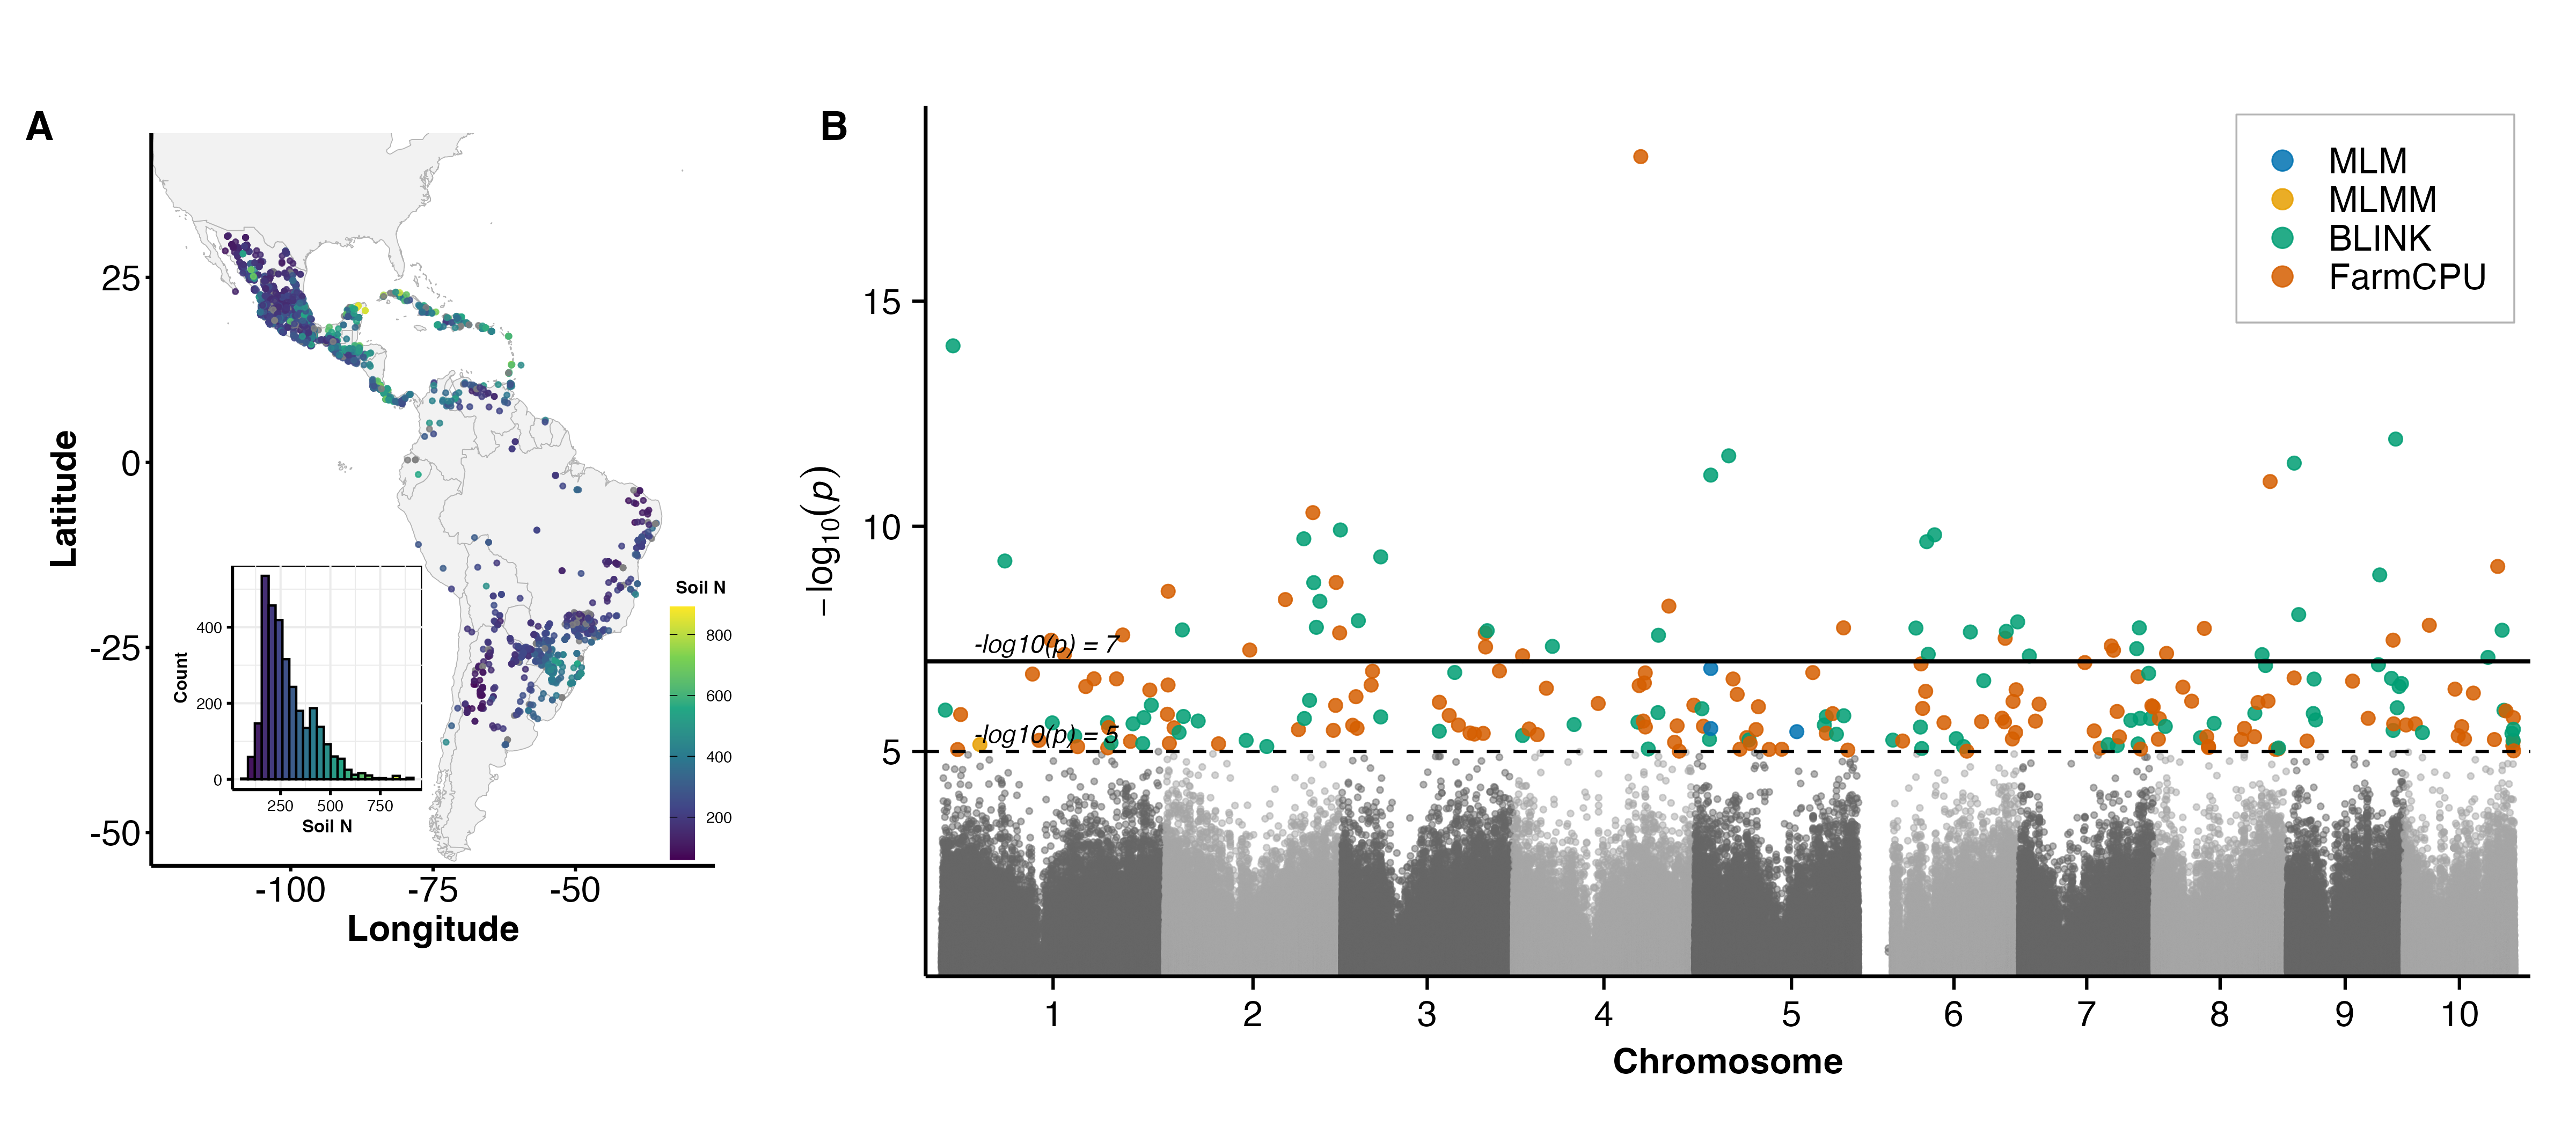
\includegraphics[width=\textwidth]{Figs/main/Fig1.png}
    \caption{Geographic distribution of soil nitrogen and genome-wide association results for soil N. \textbf{A}, Sampling locations across the Americas colored by soil N, with an inset histogram showing the soil N distribution across accessions. \textbf{B}, Manhattan plot of soil N GWAS results across chromosomes. Colored points indicate loci identified by the MLM, MLMM, BLINK, and FarmCPU models. Horizontal lines indicate suggestive and more stringent significance thresholds.}
    \label{fig:soilN_gwas}
\end{figure}


Two candidates are notable because their functions link soil nitrogen variation to amino acid metabolism. The top candidate, \textit{Zm00001eb005710}, encodes a CN hydrolase domain–containing protein. It shows a strong association with soil N ($-\log\_{10}(P) = 14.01$) and is annotated with omega-amidase/NIT2-like activity, hydrolase activity on carbon–nitrogen bonds, and roles in oxaloacetate, asparagine, and glutamine metabolism. A second candidate, \textit{Zm00001eb220040}, encodes a protein with an aspartate/glutamate/uridylate kinase domain and is associated with soil N at $-\log_{10}(P) = 11.14$. Its Gene Ontology annotations include aspartate kinase activity, amino acid biosynthesis, and threonine biosynthesis. Since aspartate kinase catalyzes an early committed step in the aspartate-family amino acid pathway, this locus is a plausible mediator of soil N effects on downstream amino acid biosynthesis (ref).

Together, these results highlight \textit{Zm00001eb220040} and \textit{Zm00001eb005710} as nitrogen-metabolism-related candidates involved in aspartate, asparagine, and glutamine metabolism. These inferences are based on annotations and GO terms rather than direct experiments and should be viewed cautiously. Nonetheless, the alignment of soil N GWAS signals with amino acid metabolism–related annotations supports a mechanistic link between environmental nitrogen availability and grain nitrogen-associated metabolic pathways.


\subsection{B64 × CML14 biparental mapping identifies candidate loci for grain asparagine accumulation}


\subsection{Skim sequencing reveals generation-specific genetic differentiation in Indian Chief and Jarvis}

To evaluate selection-associated variation in nitrogen accumulation and partitioning we utilizaed the Indian Chief and Jarvis maize population.  These populations derive from long-term recurrent selection experiments in which Jarvis Golden Prolific and Indian Chief served as open-pollinated base populations, and selection for 14 cycles targeted grain weight per plant as the sole direct criterion \citep{Moll1994}. Previous phenotypic work showed that reciprocal recurrent selection altered nitrogen allocation differently in Jarvis and Indian Chief. At nonlimiting N supply, Jarvis after 14 cycles of reciprocal recurrent selection accumulated greater grain N and showed greater post-anthesis loss of N from stover relative to the original Jarvis population. In contrast, Indian Chief after 14 cycles of reciprocal recurrent selection showed increased post-anthesis stover biomass, but had lower grain weight, lower post-anthesis loss of N from stover, and no significant increase in grain N relative to the original Indian Chief population \citep{Moll1994}.


We performed skim sequencing on 100 individuals each from the Indian Chief and Jarvis maize populations at Generations~0 and 14. Sample-level sequencing metrics matched expectations for low-coverage skim sequencing (Supplementary Fig.~\ref{fig:seq_sample_level}). Across 379 individuals, mean sequencing depth was 0.73$\times$ (median 0.72$\times$, range 0.32--1.91$\times$). Most samples had 0.5--1.0$\times$ coverage (323/379); 26 were below 0.5$\times$, 29 were between 1.0$\times$ and 1.5$\times$, and one exceeded 1.5$\times$ (Supplementary Fig.~\ref{fig:seq_sample_level}A,C). Despite the low depth, genotype recovery was high and uniform, with $\sim$59.0 million genotypes called per individual (Supplementary Fig.~\ref{fig:seq_sample_level}B). Missing data were moderate for skim sequencing, with a median of 102{,}814 missing genotypes per sample, a 95th percentile of 167{,}497, and a maximum of 328{,}163 per individual.

Variant-level summary statistics indicated that the dataset was suitable for population-level genetic analyses. (Supplementary Fig.~\ref{fig:seq_variant_level}). Per-site sequencing depth was centered near 7$\times$ across retained variants, with an interquartile range of 5–9$\times$ (Supplementary Fig.~\ref{fig:seq_variant_level}A). The minor allele frequency spectrum was skewed toward low-frequency variants, as expected for segregating breeding populations with substantial standing genetic variation (Supplementary Fig.~\ref{fig:seq_variant_level}B). Missing genotype counts declined smoothly across samples ranked by missingness, indicating that missing data were not driven by a small subset of problematic individuals (Supplementary Fig.~\ref{fig:seq_variant_level}C). Transition/transversion ratios were highly consistent across the 10 maize chromosomes (1.74–1.81; genome-wide mean 1.785; Supplementary Fig.~\ref{fig:seq_variant_level}D). After filtering, 512,667 SNPs were retained, and a linkage-disequilibrium–pruned subset of 57,568 markers was used for population-structure analyses.





Population-structure analyses showed that Indian Chief and Jarvis remained genetically differentiated after 14 generations of selection, while also exhibiting clear generation-associated shifts within each population (Fig.~\ref{fig:fig3}A). Individual ancestry profiles clustered primarily by source population, with little evidence of extensive admixture. Within each population, comparisons between Generation~0 and Generation~14 revealed shifts in inferred ancestry components, consistent with selection-driven allele-frequency changes. Principal component analysis was concordant: PC1 explained 1.32\% of the variance and primarily separated Indian Chief from Jarvis, whereas PC2 explained 0.83\% and further distinguished Generation~0 from Generation~14 within each population (Fig.~\ref{fig:fig3}B). Thus, long-term selection preserved the ancestral population identities of Indian Chief and Jarvis while generating detectable genome-wide differentiation between ancestral and selected generations.

Shared-SNP summaries provided an additional view of temporal and between-population shifts in allele composition (Fig.~\ref{fig:fig3}C,D). Within populations, Generation~0 individuals shared more SNPs with Generation~14 than vice versa. In Indian Chief, the mean proportion of shared SNPs was ~0.799 for Generation~0 relative to Generation~14, versus 0.371 for Generation~14 relative to Generation~0; in Jarvis, the values were ~0.726 and 0.483, respectively (Fig.~\ref{fig:fig3}C). This asymmetry indicates that many ancestral alleles persisted into Generation~14, while selected-generation individuals also carried generation-enriched alleles that were relatively rare in Generation~0.


\begin{figure}[!htbp]
    \centering
    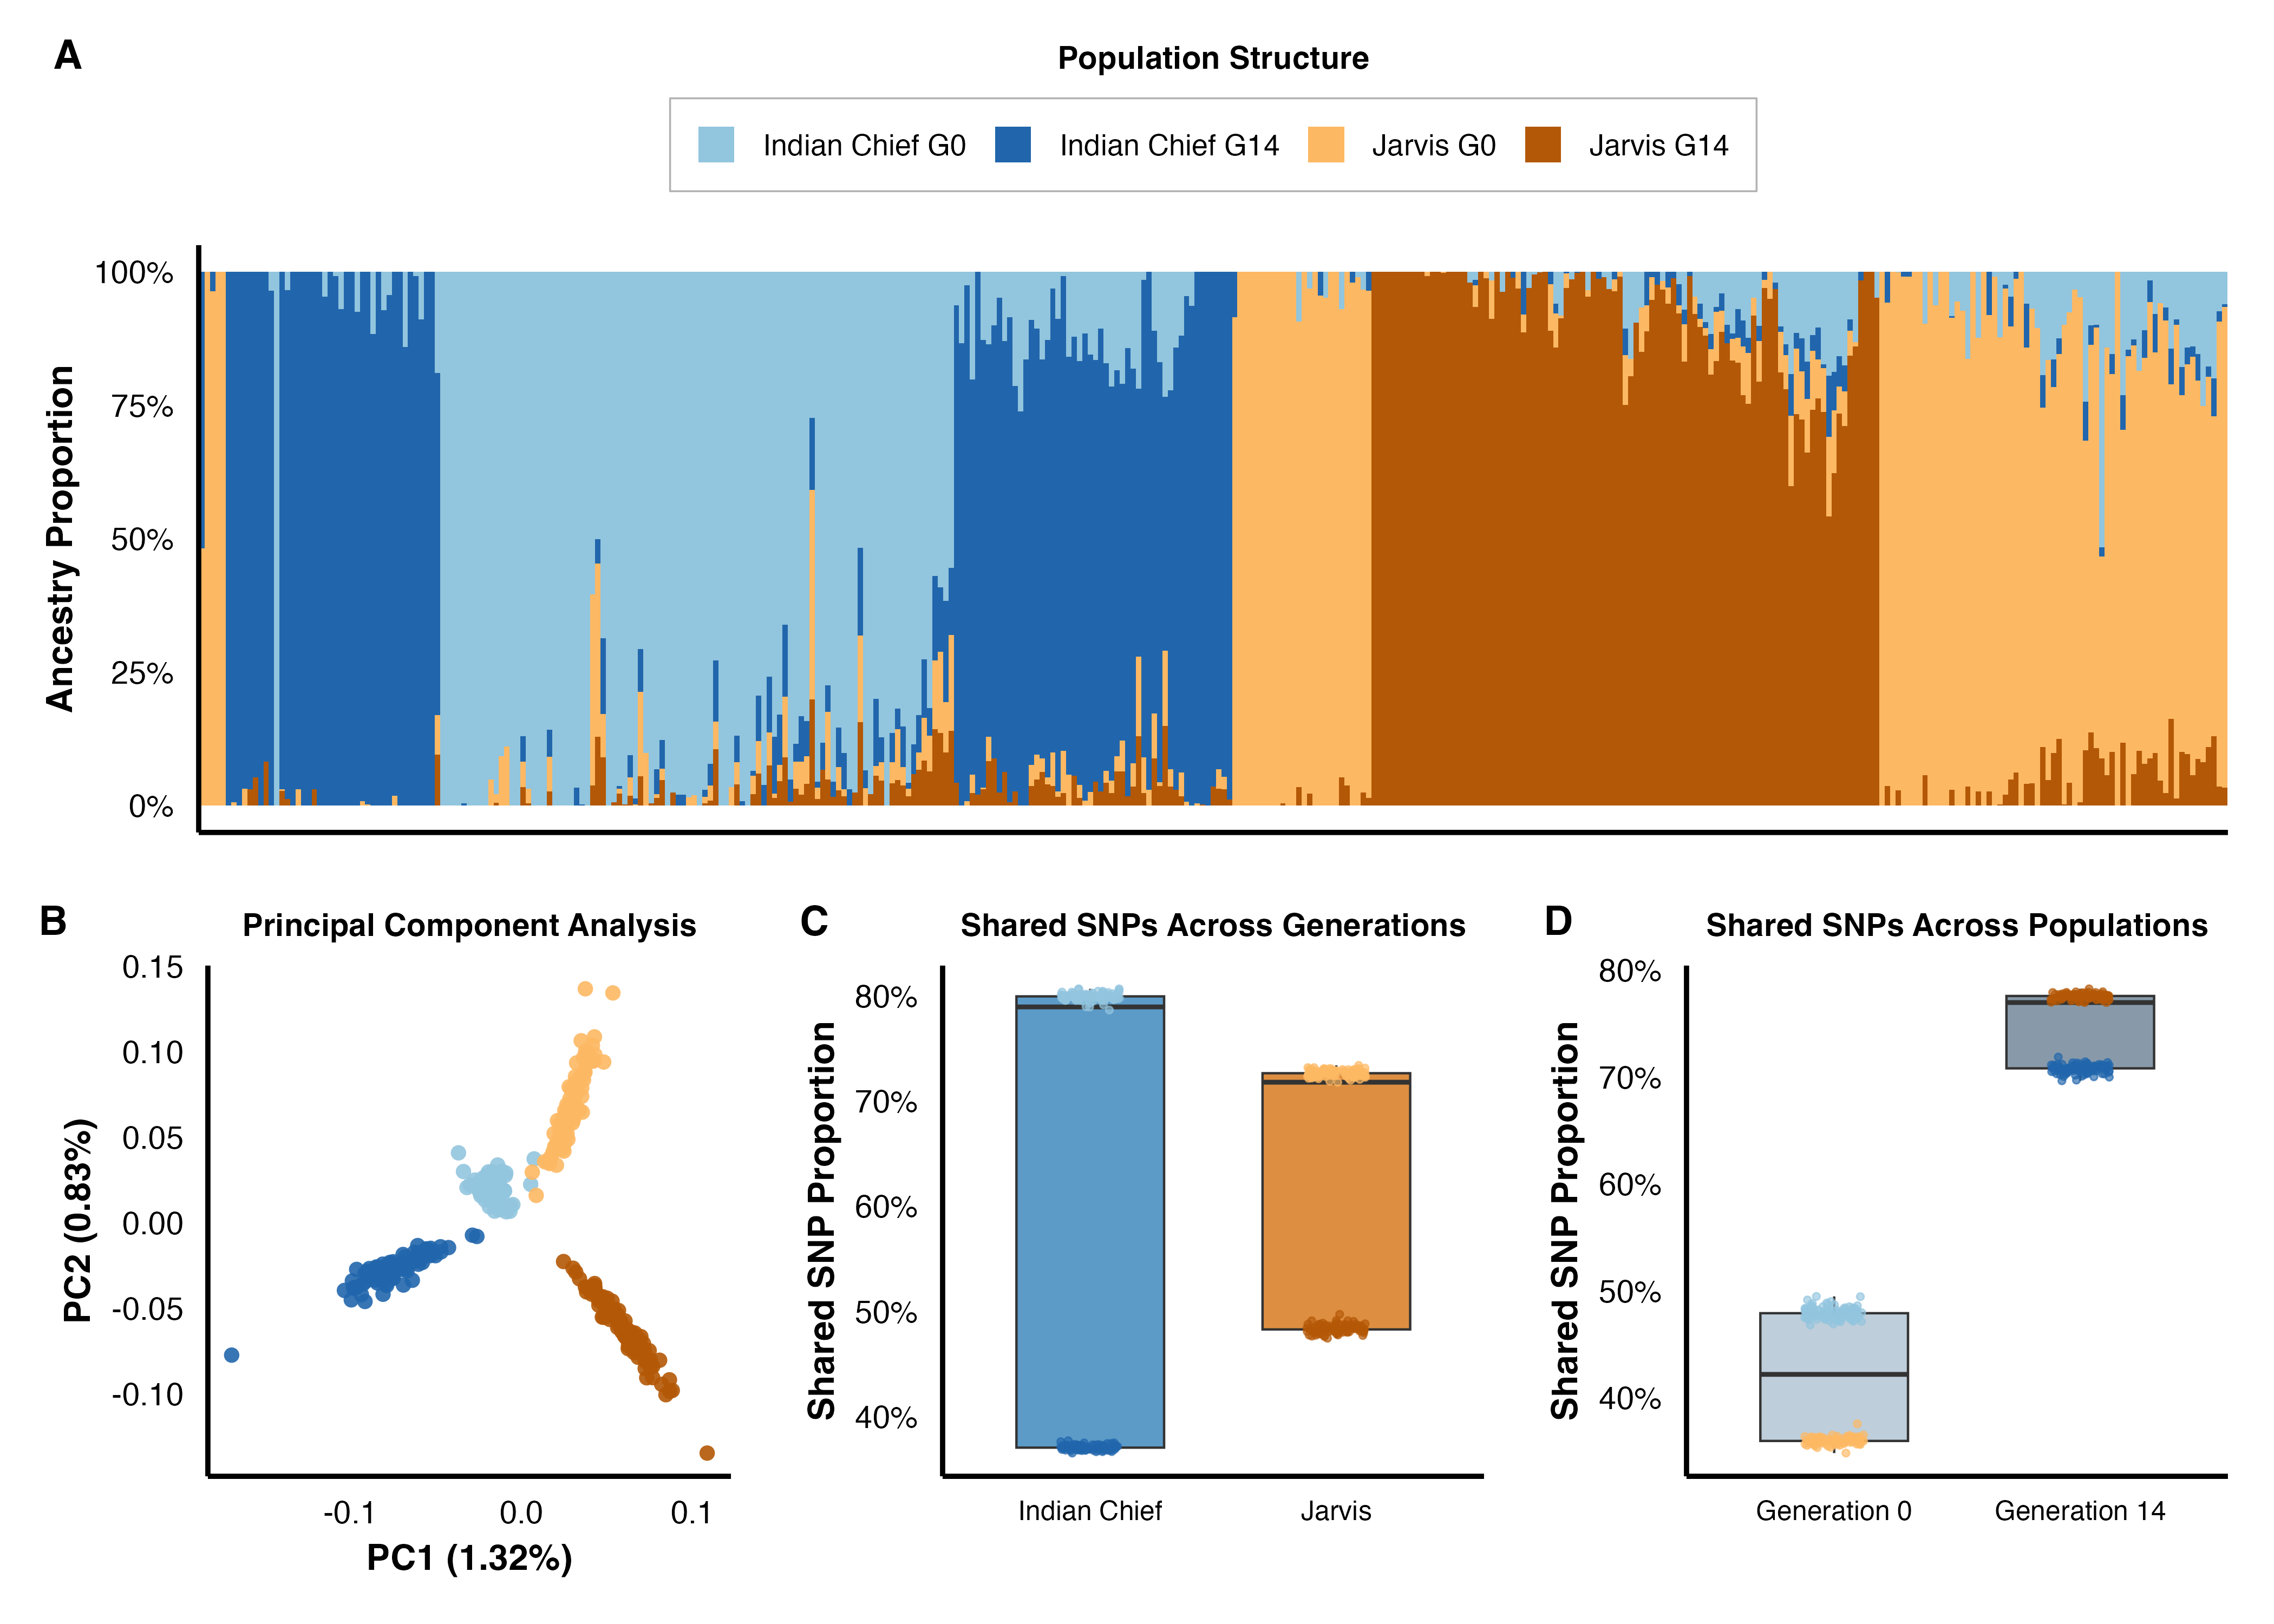
\includegraphics[width=\textwidth]{Figs/main/Fig3.png}
    \caption{Skim sequencing reveals generation-specific genetic differentiation in Indian Chief and Jarvis. \textbf{A}, Population structure inferred from the LD-pruned SNP set, with ancestry proportions shown for Indian Chief Generation~0, Indian Chief Generation~14, Jarvis Generation~0, and Jarvis Generation~14. \textbf{B}, Principal component analysis of the same individuals and marker set. \textbf{C}, Proportion of SNPs shared across generations within each population. \textbf{D}, Proportion of SNPs shared across populations within each generation.}
    \label{fig:fig3}
\end{figure}

Between populations, patterns differed from those within populations. Generation~14 individuals shared a higher proportion of SNPs between Indian Chief and Jarvis than did Generation~0 individuals, with mean proportions of ~0.742 and 0.420, respectively (Fig.~\ref{fig:fig3}D). Thus, long-term selection increased the fraction of alleles shared between the two selected populations, even though Indian Chief and Jarvis remained clearly differentiated in structure and PCA. Overall, 14 selection cycles markedly reshaped allele frequencies within each population, increased allelic overlap between generations, yet preserved broad genomic differentiation between Indian Chief and Jarvis.


\subsection{Population selection scans implicate protein turnover and amino acid remodeling in population-specific N allocation}

Free amino acid profiles revealed population-specific changes in proline accumulation between Cycle~0 and Cycle~14. In Indian Chief, proline was higher in Cycle~14 than in Cycle~0, whereas Jarvis showed the opposite pattern, with higher proline in Cycle~0 and reduced proline by Cycle~14 (Fig.~\ref{fig:fig4}). This reciprocal pattern suggests that long-term reciprocal recurrent selection altered free amino acid pools differently in the two populations. However, proline alone should not be interpreted as a direct measure of N remobilization. Rather, the proline shift is consistent with broader remodeling of nitrogen-containing metabolites during selection.

\begin{figure}[!htbp]
    \centering
    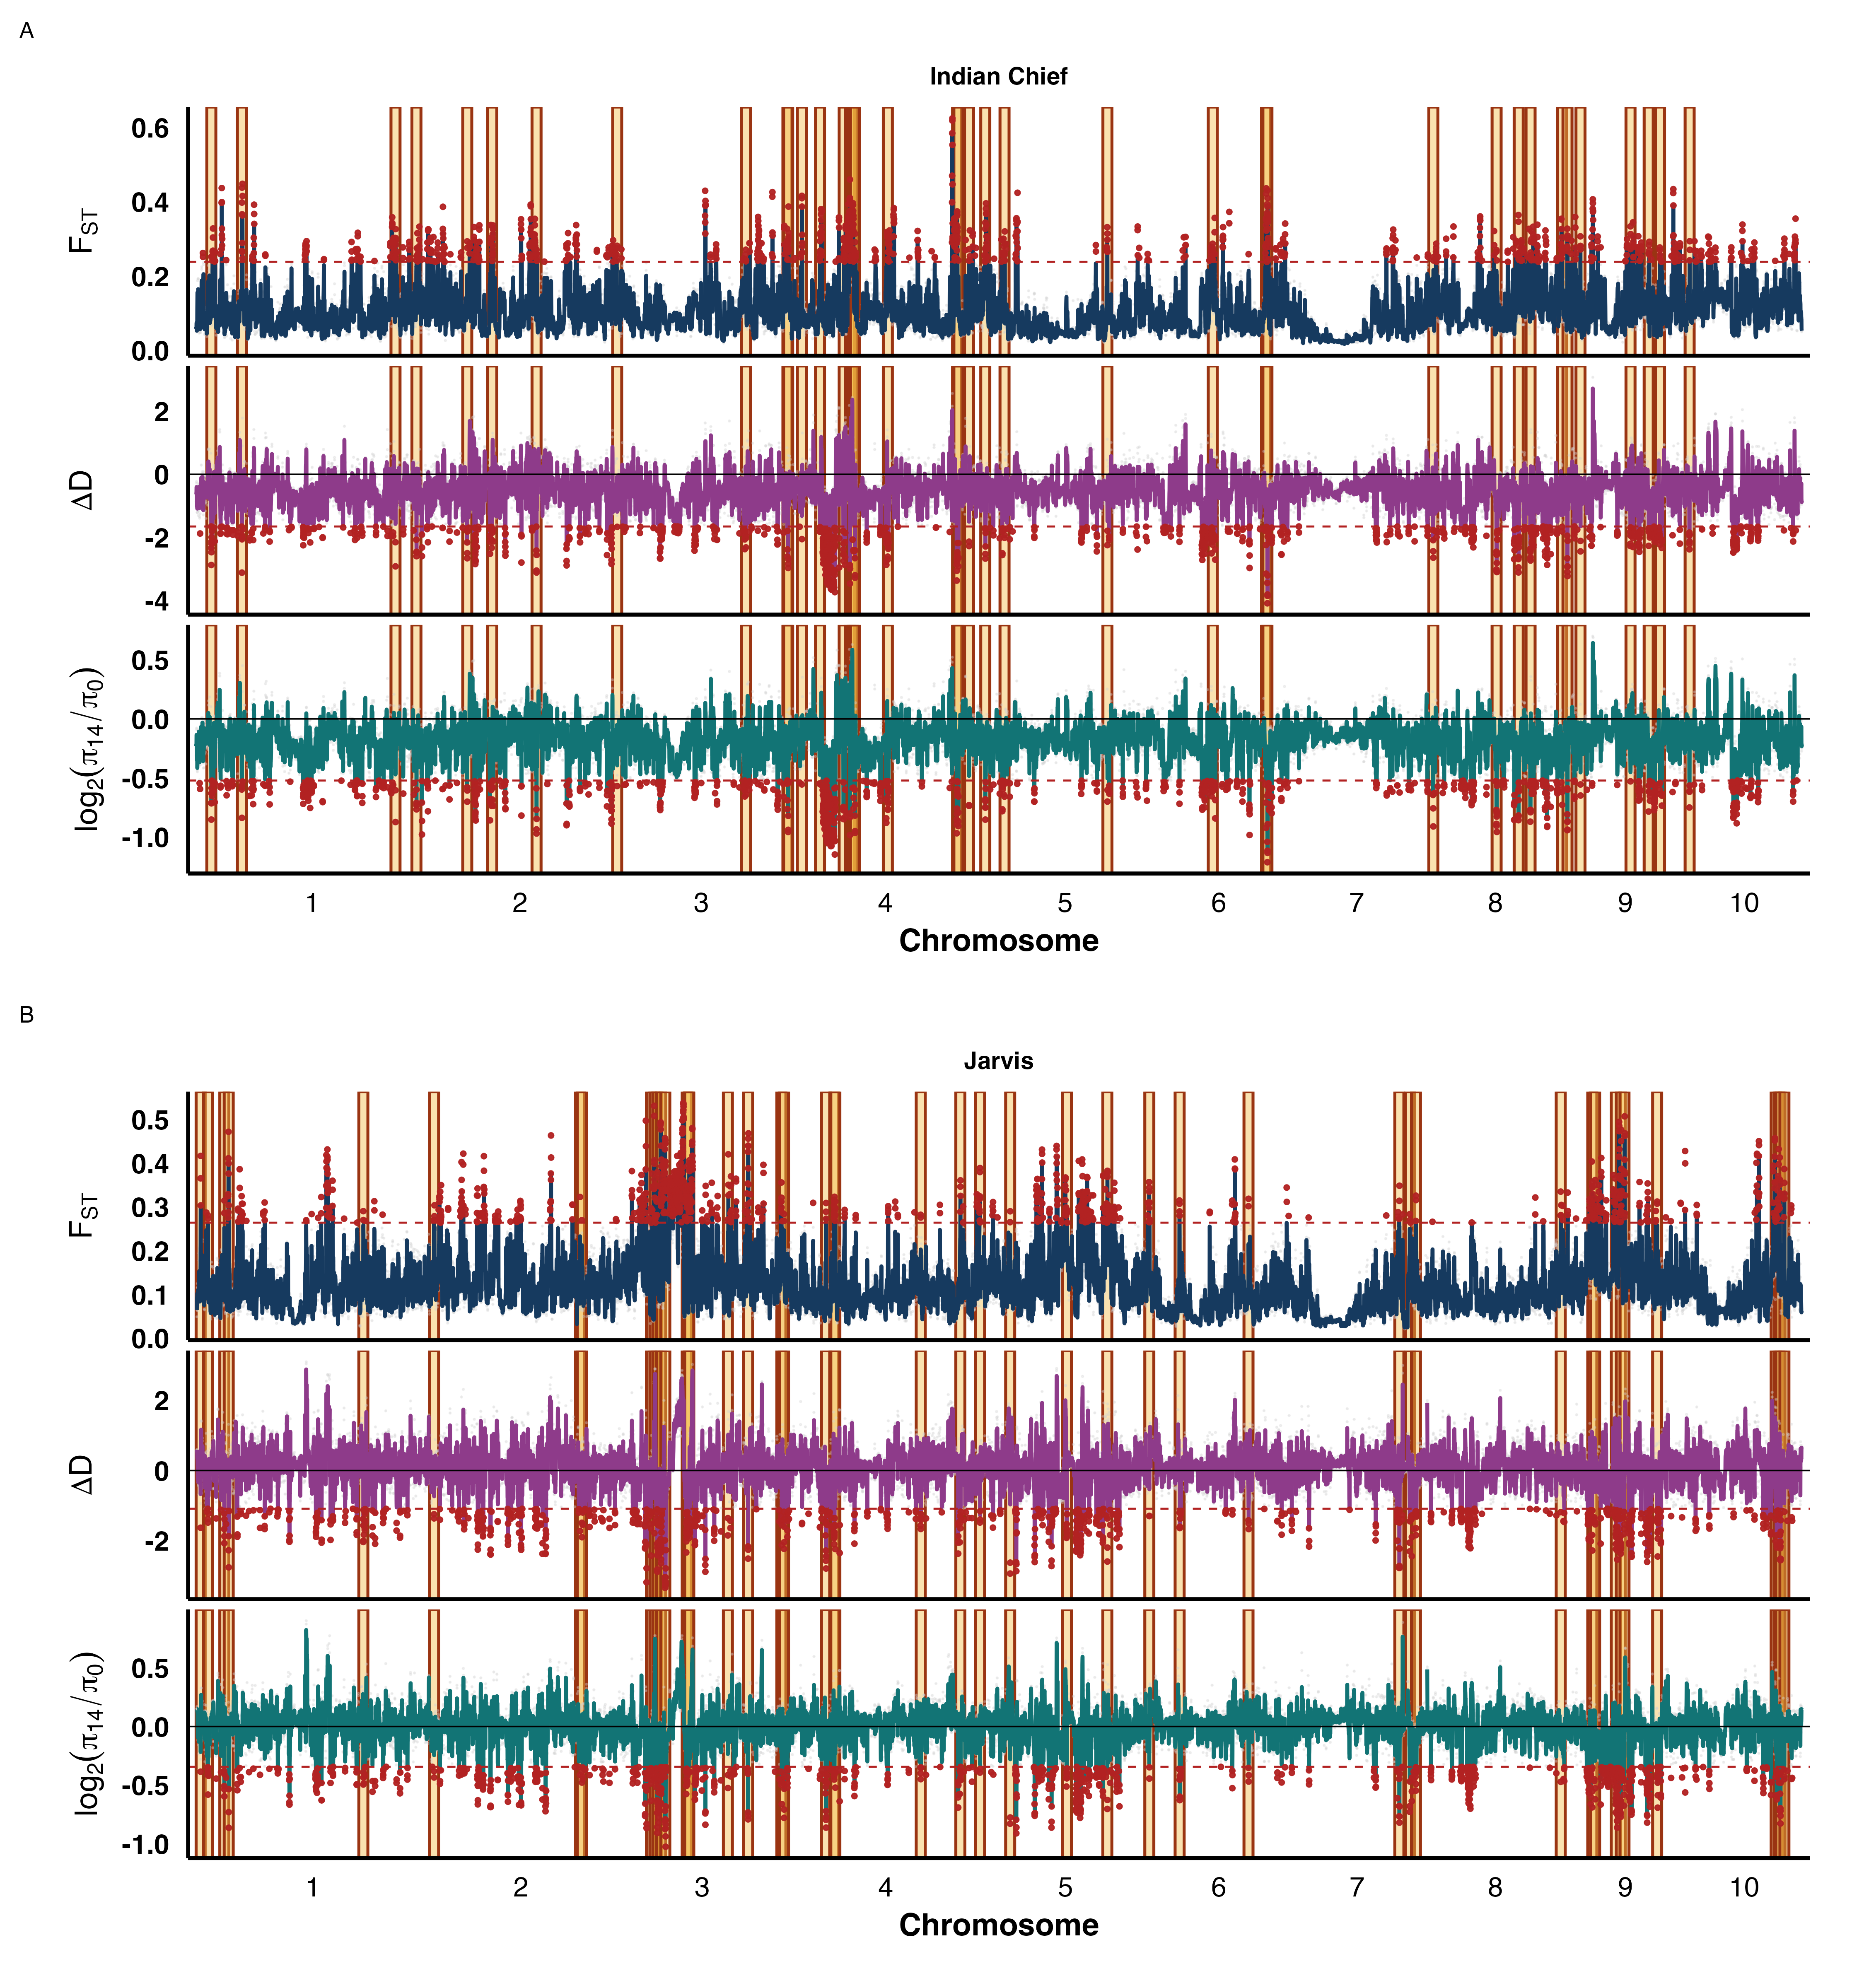
\includegraphics[width=\textwidth]{Figs/main/Fig4.png}
    \caption{Genome-wide scans of population differentiation and diversity changes between Generation~0 and Generation~14 in Indian Chief and Jarvis. \textbf{A}, Indian Chief. \textbf{B}, Jarvis. Tracks show $F_{ST}$, $\Delta$ Tajima's $D$, and $\log_2(\pi_{G14}/\pi_{G0})$ across the genome. Shaded vertical bands indicate candidate regions supported by all three summary statistics under the empirical 5\% threshold scheme, defined as the top 5\% of $F_{ST}$ values together with the bottom 5\% of $\Delta$ Tajima's $D$ and $\log_2(\pi_{G14}/\pi_{G0})$ values.}
    \label{fig:fig4}
\end{figure}

This interpretation agrees with previous phenotypic work on the same recurrent-selection material. Under reciprocal recurrent selection, Jarvis Cycle~14 showed greater grain N and greater post-anthesis loss of N from stover relative to the original Jarvis population, consistent with stronger remobilization of vegetative N into grain. In contrast, Indian Chief Cycle~14 showed increased post-anthesis stover biomass, but did not show a significant increase in grain N and had reduced post-anthesis loss of N from stover relative to the original Indian Chief population \citep{Moll1994}. Thus, the contrasting proline profiles may reflect different N-allocation strategies: Jarvis Cycle~14 appears more consistent with N movement toward grain, whereas Indian Chief Cycle~14 appears more consistent with retention or accumulation of N-rich pools in vegetative tissues.

Genome-wide selection scans further supported a role for protein turnover and nutrient recycling in Indian Chief. Across the candidate sets from $F_{ST}$, nucleotide diversity, and Tajima's $D$, Indian Chief contained one overlapping gene, \textit{Zm00001eb372060}, annotated as an autophagy-related protein, whereas Jarvis had no gene shared across all three scan classes (Supplementary Table~\ref{tab:selection_candidate_go}). Autophagy is directly relevant to N remobilization because it contributes to degradation and recycling of cellular proteins and organellar material during senescence and nutrient redistribution. Therefore, the overlap of an autophagy-related gene in Indian Chief provides a biologically plausible candidate linking selection-associated differentiation with altered N recycling.

Additional annotated candidates reinforced this protein-turnover theme. Indian Chief candidate regions included genes annotated as cysteine proteinases, ubiquitin-like proteases, E3 ubiquitin ligases, Cullin-related proteins, and proteasome-associated functions, including terms such as proteolysis, ubiquitin-dependent protein catabolic process, protein ubiquitination, and proteasome-mediated ubiquitin-dependent protein catabolic process. Indian Chief also contained a candidate annotated with cellular response to nitrogen starvation and chlorophyll catabolic process, connecting selection signatures with nutrient stress, chloroplast turnover, and senescence-associated recycling. Jarvis candidate regions also contained protein-turnover genes, including an ATG8-interacting protein, aspartyl protease, cytosol aminopeptidase, Cullin-related genes, HECT-type E3 ubiquitin transferase, and ubiquitin/deubiquitination-related annotations. However, unlike Indian Chief, these candidates did not converge into a single gene shared across all three selection statistics.

Together, the amino acid and selection-scan results suggest that reciprocal recurrent selection altered N allocation through different routes in Indian Chief and Jarvis. In Jarvis, reduced Cycle~14 proline together with prior evidence for increased grain N is consistent with stronger movement or utilization of N-containing compounds during grain filling. In Indian Chief, increased Cycle~14 proline and the presence of an overlapping autophagy-related candidate suggest a distinct remodeling of protein turnover and amino acid pools, potentially associated with vegetative N retention and recycling. These candidate-gene interpretations are based on GO annotations and selection-scan overlap, and therefore should be treated as hypotheses for future functional validation rather than direct proof of causal remobilization mechanisms.


\subsection{Total Protein and Nitrogen Proxy GWAS}
Total protein can reasonably be calculated from the sum of each PBAA. Our GWAS of total PBAA yielded 16 significant SNPs that contained 501 unique candidate genes within a 200kb region. The majority of these associations were detected using the BLINK and FarmCPU models, with only two SNPs identified by MLMM. Notably, one SNP (7-5322774) was consistently identified across all three models. Though grain protein accounts for a large proportion of the nitrogen found in the grain, it may not accurately represent the levels of nitrogen present due to variances in amino acid composition and levels of free amino acids. For this reason we opted to calculate a proxy nitrogen content that takes these factors into account. GWAS of proxy nitrogen also yielded 16 significant SNPs, though only four overlapped with those identified for total protein. These proxy nitrogen SNPs were associated with 489 candidate genes, 173 of which were also found in the total protein results. As with total protein, most associations were identified using BLINK and FarmCPU. One SNP (1-80777231) was identified by all three models for proxy nitrogen and was also detected in both BLINK and MLMM for total protein. These results suggest that while total protein and proxy nitrogen share some genetic architecture, they also capture distinct aspects of nitrogen-related variation. 



\subsection{Free Amino Acid GWAS}
In addition to the total PBAA and proxy nitrogen traits, we evaluated 110 additional traits related to free amino acid (FAA) accumulation in maize grain. These included the absolute concentrations of all 20 proteinogenic amino acids, their relative abundances (as proportions of total FAAs), and a set of biochemical ratios comparing individual amino acids and their metabolic families. Across the 112 traits, we identified a total of XX,XXX significant SNPs using four GWAS models: BLINK, FarmCPU, MLM, and MLMM. After applying FDR correction, XX,XXX SNPs remained significant, corresponding to XX,XXX candidate genes. To better understand the genetic basis of nitrogen accumulation in maize grain, we focused on traits related to asparagine (Asn), aspartate (Asp), glutamine (Gln), and glutamate (Glu), given their central roles in nitrogen assimilation and transport. In addition to their absolute and relative abundances, we analyzed 11 biochemical ratios involving the glutamate and aspartate amino acid families. Across these 19 traits, we detected 649 significant SNPs: 478 from FarmCPU, 220 from BLINK, 21 from MLMM, and 16 from MLM. Within a 200 kb window of these SNPs, we identified 14,639 candidate genes.



\section{Methods}\label{methods}

\subsection{Germplasm used}
\subsubsection{Maize Landraces}
The maize landraces discussed by Romero Navarro et al. (2017, ref) come from the CIMMYT International Germplasm Bank collection, which contains over 24,000 accessions of traditional maize varieties primarily from North, Central, and South America. They characterized a core collection of 3,511 genotypes based on availability of accurate geographic coordinates and complete environmental data for their collection locations. These landraces are genotyped using genotyping-by-sequencing (GBS) at about 2X coverage, with SNP calling and imputation for analysis. The population represents a geographically and genetically diverse panel that serves as an important resource for studying environmental adaptation like soil nitrogen (N) availability.
How were they grown when they were phenotyped?

\subsubsection{Indian Chief and Jarvis (IC and J)  }
We worked with two open-pollinated maize populations Indian Chief (IC) and Jarvis (J) from Moll et al. (1994, ref) that underwent reciprocal recurrent selection for 14 generations for grain yield. Beginning from base populations (G₀), each cycle involved intercrossing the best families selected on hybrid (ICxJ) performance and advancing through a selfed recombination nursery. 
How were they grown in 2025? This is relevant for the AA profiling I am doing 

\subsubsection{The Goodman-Buckler Maize Association Panel}
The Goodman-Buckler maize association panel (Flint-Garcia et al., 2005)  was grown at Genetics Farm near Columbia Missouri in 2017 and 2018 in two replicates each, in a randomized complete block design. Of the 282 lines in this panel, only 279 were grown successfully. 13 kernels of each line were planted in a 10 foot row and self-pollinated. At full physiological maturity, the pollinated ears were harvested, husk leaves were removed, and were subsequently dried at 105 degrees fahrenheit and <20 relative humidity for 5 days to remove moisture from the grain. Ears from each line in each rep and year were shelled and bulked to form four representative composite grain samples for each of the 279 lines. For phenotypic evaluation, 25 random seeds were selected from each bulked sample to be ground and prepared for amino acid extraction and quantification

\subsubsection{Bi-parental Mapping Population}
The bi-parental QTL mapping population was developed by crossing the two inbred lines of the Goodman-Buckler Association Panel with the lowest and highest free Asn accumulation in the grain, B64 and CML14, respectively. F2:3 families were grown in two complete randomized blocks in 2024 at Genetics Farm near Columbia Missouri. For each plot, 13 kernels were planted in a 10-foot row and sib-pollinated to produce three ears. At full physiological maturity, the pollinated ears were harvested, husk leaves were removed, and ears were subsequently dried at 41 degrees Celsius and 20\% relative humidity for 5 days to remove moisture from the grain. From each ear, 10 representative kernels were sampled then bulked, ground, and prepared for amino acid extraction and quantification.


\subsection{Phenotypic Evaluation}
\subsubsection{Grain/Stover Nitrogen}
Grain and stover N concentration for all IC and J lines was determined for the base generation (G₀) and the 14ᵗʰ cycle of selection (G₁₄) by Moll et al, (1994, ref). At a high fertilizer rate of 224 kgNha⁻¹, the J14 produced heavier kernels and a higher grain N concentration than the original J0 line. Post anthesis uptake from the soil supplied almost all of that extra N while the amount of nitrogen remobilised from stover to grain remained unchanged. The I14 behaved differently though. Vegetative biomass increased, but grain weight and grain N concentration stayed at the G₀ level. Loss of nitrogen from stover after flowering fell below that of the baseline, so more N was retained in stems and leaves and less reached the grain. Fourteen cycles of selection therefore raised grain N in J by drawing in more N after flowering, whereas the IC diverted N toward vegetative tissue and left grain N unchanged (ref).

\subsubsection{Soil Nitrogen}
The analyzed phenotypes include total N in the soil (TN) and nitrate deposition (NHx, which includes NH3 and NH4+). N data were derived from the top 0-5 cm of the soil, representing the active root zone for nutrient uptake, using ISRIC data sets (International Soil Reference and Information Center). Historical nitrate deposition data (NHx) from 1983 was also sourced from ISRIC to understand its relationship with nutrient uptake. 

\subsubsection{Amino Acid Profiling}
PBAAs were extracted and quantified as described in Yobi and Angelovici (2018). This protocol utilizes microscale protein hydrolysis and absolute quantification using multiple reaction monitoring-based liquid chromatography–tandem mass spectrometry detection. During acid hydrolysis, Gln and Asn are converted into Glu and Asp, respectively. Therefore, we denote both Gln and Glu as Glx and Asn and Asp as Asx. During the extraction, Trp and Cys were fully destroyed and Gly was poorly detected, therefore these three amino acids were excluded from the dataset. In total, 15 PBAAs were analyzed to represent 17 PBAAs. FAAs were extracted and quantified as described in (Gu et al., 2007). Unlike the protocol above, all 20 proteinogenic amino acids were independently and successfully detected using UPLC-MS/MS.


\subsection{Sequencing and Genotyping}
\subsubsection{Indian Chief and Jarvis }
Genomic DNA was isolated from young leaf tissue of 96 individuals each from the IndianChief base generation (I01), IndianChief 14th generation (I14), J base generation (J01) and J 14th generation (J14) populations generated after 14 cycles of reciprocal‑recurrent selected for increased yield (ref). Illumina libraries for forward and reverse reads (2× 150bp) were constructed and sequenced on a NovaSeq6000. Raw base‑call files were demultiplexed with fqtk version 0.3.1 (ref), yielding four 96‑sample plates for each of the varieties and generations (Supplementary Table S1).
Adapter trimming and quality filtering were performed with fastp version 0.23.4 (ref). FastQC version 0.12.1 confirmed removal of adapter sequences. Trimmed reads were aligned to the B73 NAM reference genome (RefGen\_v5; GCF\_902167145.1) from NCBI using BWA‑MEM version 0.7.18 with default parameters. Alignments were coordinate sorted, and duplicate fragments were collapsed with PicardMarkDuplicates version 3.1.1. Read groups were reassigned to standardized sample identifiers (I01, I14, J01, J14) with PicardAddOrReplaceReadGroups.
Genotype calling was performed using GATK version 4.5.0.0, following the GATK Best Practices workflow for joint genotyping (ref). Joint genotyping was conducted chromosome‑wise with GATKCombineGVCFs followed by GenotypeGVCFs, producing 10 per‑chromosome VCFs that were merged into a cohort VCF containing 80,728,251 raw variant sites. Five samples exhibiting <0.15× depth and/or <50\% properly‑paired reads (I14\_A07, I14\_B06, I14\_D05, I14\_F12, J14\_H11) were removed, leaving 379 high‑quality genomes (Supplementary Table 1). Genome‑wide coverage, assessed with PicardCollectWgsMetrics, averaged 0.28× (I01), 0.38× (I14), 0.32× (J01) and 0.37× (J14) (Supplementary Fig S1). Hard filters recommended by GATK were applied separately to SNPs and indels (QD<2.0, FS>60.0, MQ<40.0, MQRankSum<–12.5, ReadPosRankSum<–8.0, SOR>3.0 for SNPs; analogous indel thresholds). Variants failing any filter were removed, yielding 59,199,563 high‑confidence sites (52,543,238 SNPs; 6,656,325 indels) distributed across the ten maize chromosomes and scaffolds (Supplementary Table S2). 
The Goodman-Buckler Maize Association Panel

\subsubsection{The Goodman-Buckler maize association panel}
The Goodman-Buckler maize association panel had been previously genotyped with both the Illumina MaizeSNP50 BeadChip (Cook et al., 2012) and with genotyping-by-sequencing (GBS) method (Elshire et al., 2011) as described in (Lipka et al., (2013). We filtered SNPs by minor allele frequency greater than 0.05 prior to analysis. HAPPI GWAS utilizes GAPIT MLMM, FarmCPU, and BLINK models to conduct univariate GWAS. Following the GWAS, we used false discovery rate (FDR) to correct the multiple hypothesis testing problem at 5\%. Using the Maize AGP\_V5, we identified candidate genes within 25kb on either side of SNPs with a p value of less than 0.001. 

\subsubsection{Bi-parental Mapping Population}
Leaf tissues were collected from F2 plants and lyophillized prior to DNA extraction and genotyping using the mid-density temperate corn panel by Agriplex Genomics (Cleveland, OH).

\subsection{Population analyses}
\subsubsection{FST}
The IC and J populations were sequenced at low pass (~0.8x) using TWIST BioSciences (ref). For this, we utilized genotype likelihoods to estimate site‑frequency spectra and F$_{ST}$ in the probabilistic framework using ANGSD  version 0.941 (ref). ANGSD integrates genotype likelihoods over read depth and base quality, producing unbiased F$_{ST}$ estimates even when per‑sample coverage is <1x. Windows of 100kb with a 10kb step were used to smooth site‑wise estimates. The top 1\% windows were treated as outliers and were retained for further analysis.  

\subsubsection{Genome-wide association Studies}
\paragraph{Environment GWAS}
GWAS was performed on maize landraces (n = 3,511) using four GWAS models: MLM, MLMM, BLINK and FarmCPU. Approximately 495,755 SNPs for maize landraces. The maize genotype was based on the Zm-B73-REFERENCE-NAM-5.0 genome assembly. Candidate genes located within 25 kb maize landraces were identified using the MaizeGDB, Phytozome, and Arabidopsis databases. 

\paragraph{Metabolite GWAS}
Using the same pipeline described above for the envGWAS, we performed metabolite GWAS using the Goodman-Buckler Association Panel (n-278). In total, XXX SNPs were used to evaluate 110 traits for FAAs and 77 traits for PBAAs including absolute composition, total composition, relative composition, and various biochemical ratios. Prior to analysis, best linear unbiased predictions or BLUPs were calculated for each trait. For the metabolite GWAS, we used a GAPIT pipeline based on Holistic Analysis with Pre- and Post-Integration, or HAPPI GWAS. This pipeline, as described in (Slaten et al., 2020), removes outliers, optimizes transformation, and calculates BLUPs prior to the association study. 

To estimate the nitrogen content of the Goodman-Buckler maize association panel, we calculated the respective percentage of mass occupied by nitrogen in the 20 proteinogenic amino acids. Across the 4 composite samples, we multiplied the quantity of each amino acid in μg/mg by the calculated \% nitrogen mass for that amino acid to solve for the  quantity of nitrogen in μg/mg. We added the totals for each of the 20 proteinogenic amino acids together for the free amino acids as well as the quantified protein bound amino acids to find total approximated nitrogen content in each composite sample. 

\[
\%N_X =
\left(
\frac{n_{N,X}\times M_N}{M_X}
\right)\times 100
\]

where,
\[
M_X = \text{molar mass of amino acid } X
\]

\[
M_N = \text{molar mass of nitrogen}
\]

\[
n_{N,X} = \text{number of nitrogen atoms in amino acid } X
\]

Finally,
\[
N_X\;(\mu g/mg) =
\left(
\frac{n_{N,X}\times M_N}{M_X}
\right)
\times AA_X\;(\mu g/mg)
\]



We used these total proxy nitrogen (TPN) amounts for each composite sample to calculate the Best Linear Unbiased prediction (BLUP) before performing the GWAS as described above. We used a false discovery rate (FDR) to correct the multiple hypothesis testing problem at 5\%. Using the MaizeMine tool on MaizeGDB, we identified candidate genes within 100kb on either side of SNPs with a p value of less than 0.001. 

\paragraph{Quantitative Trait Loci Mapping}
We began with 2490 markers in total and following filtering of failed, monomorphic, and heterozygous markers 611 were used for the analysis. Markers were re-coded to be compatible with the r/qtl package used for mapping. Each allele was re-coded to AA to correspond with the allele associated with B64, BB for CML14, and AB if heterozygous. Best Linear Unbiased Predictions of absolute free aspartate content were calculated and used to construct the genetic map. To ensure quality of the genetic map, markers with more than 10\% inconclusive genotyping results were excluded and segregation ratios were checked to identify and remedy potential switched alleles. Linkage groups were formed by calculating max recombination fraction at 0.35 and minimum LOD at 15. Ultimately, one linkage group required manual separation and subsequent re-calculation of recombination fraction and LOD to produce an accurate genetic map to reflect the 10 chromosomes of maize. QTL scans were performed and significance thresholds were established at a=0.05 using 1000 permutations and Haley-Knott regression.

\section{Data availability}
All scripts and parameter files used in the pipeline are available at the github repository: https://github.com/nirwan1265/Grain\_N\_remobilization.


\section{Discussion}\label{sec12}

Discussions should be brief and focused. In some disciplines use of Discussion or `Conclusion' is interchangeable. It is not mandatory to use both. Some journals prefer a section `Results and Discussion' followed by a section `Conclusion'. Please refer to Journal-level guidance for any specific requirements. 

\section{Conclusion}\label{sec13}

Conclusions may be used to restate your hypothesis or research question, restate your major findings, explain the relevance and the added value of your work, highlight any limitations of your study, describe future directions for research and recommendations. 

In some disciplines use of Discussion or 'Conclusion' is interchangeable. It is not mandatory to use both. Please refer to Journal-level guidance for any specific requirements. 

\backmatter

\bmhead{Supplementary information}

If your article has accompanying supplementary file/s please state so here. 

Authors reporting data from electrophoretic gels and blots should supply the full unprocessed scans for key as part of their Supplementary information. This may be requested by the editorial team/s if it is missing.

Please refer to Journal-level guidance for any specific requirements.

\bmhead{Acknowledgements}

Acknowledgements are not compulsory. Where included they should be brief. Grant or contribution numbers may be acknowledged.

Please refer to Journal-level guidance for any specific requirements.

\section*{Declarations}

Some journals require declarations to be submitted in a standardised format. Please check the Instructions for Authors of the journal to which you are submitting to see if you need to complete this section. If yes, your manuscript must contain the following sections under the heading `Declarations':

\begin{itemize}
\item Funding
\item Conflict of interest/Competing interests (check journal-specific guidelines for which heading to use)
\item Ethics approval and consent to participate
\item Consent for publication
\item Data availability 
\item Materials availability
\item Code availability 
\item Author contribution
\end{itemize}

\noindent
If any of the sections are not relevant to your manuscript, please include the heading and write `Not applicable' for that section. 

%%===================================================%%
%% For presentation purpose, we have included        %%
%% \bigskip command. Please ignore this.             %%
%%===================================================%%
\bigskip
\begin{flushleft}%
Editorial Policies for:

\bigskip\noindent
Springer journals and proceedings: \url{https://www.springer.com/gp/editorial-policies}

\bigskip\noindent
Nature Portfolio journals: \url{https://www.nature.com/nature-research/editorial-policies}

\bigskip\noindent
\textit{Scientific Reports}: \url{https://www.nature.com/srep/journal-policies/editorial-policies}

\bigskip\noindent
BMC journals: \url{https://www.biomedcentral.com/getpublished/editorial-policies}
\end{flushleft}

\begin{appendices}

\section{Section title of first appendix}\label{secA1}

An appendix contains supplementary information that is not an essential part of the text itself but which may be helpful in providing a more comprehensive understanding of the research problem or it is information that is too cumbersome to be included in the body of the paper.

%%=============================================%%
%% For submissions to Nature Portfolio Journals %%
%% please use the heading ``Extended Data''.   %%
%%=============================================%%

%%=============================================================%%
%% Sample for another appendix section			       %%
%%=============================================================%%

%% \section{Example of another appendix section}\label{secA2}%
%% Appendices may be used for helpful, supporting or essential material that would otherwise 
%% clutter, break up or be distracting to the text. Appendices can consist of sections, figures, 
%% tables and equations etc.

\end{appendices}

%%===========================================================================================%%
%% If you are submitting to one of the Nature Portfolio journals, using the eJP submission   %%
%% system, please include the references within the manuscript file itself. You may do this  %%
%% by copying the reference list from your .bbl file, paste it into the main manuscript .tex %%
%% file, and delete the associated \verb+\bibliography+ commands.                            %%
%%===========================================================================================%%

\bibliography{sn-bibliography}% common bib file
%% if required, the content of .bbl file can be included here once bbl is generated
%%\input sn-article.bbl

\end{document}
